\section{Introduction}
\label{sec:intro}

A benchmark paper typically reports a table: model, accuracy, robustness delta, image-reliance score. Medical VLMs are increasingly proposed for chest X-ray interpretation~\citep{chen2024chexagent,sellergren2025medgemma,bai2025qwen25vl}, and each new release is accompanied by such a table. A reader infers that the model with the higher reliance score uses the image more, that the model with the smaller degradation delta is more robust, and that a model validated in one hospital will behave comparably in another. Every one of those inferences requires a precondition that is almost never stated, and in a 270,324-call evaluation spanning three datasets and six models we found that violating each precondition \emph{reverses} the conclusion.

\textbf{Reversal 1 (responsiveness).} On PadChest, five of six models show a blank-control contrast of essentially zero: replace the radiograph with a uniform gray square and 89--100\% of replies are byte-identical. The natural reading is ``these models ignore the foreign image.'' The defensible reading is different: those same models emit \textbf{1--20 distinct answers for 1,500 distinct radiographs}. There is no variation to explain. Restricting to the 265 studies that carry at least one disease label does not rescue the reading---five models still collapse to 1--8 distinct answers. Reliance is \emph{unidentifiable}, not zero. The distinction matters: a benchmark that reports ``reliance $\approx 0$'' invites the conclusion that the model is robust to image corruption, when the model is not responding to any image at all.

\textbf{Reversal 2 (null model).} On Open-i, Qwen3-VL's blank control gives a mean Jaccard of 0.091 against the real report---an apparently strong grounding signal of the kind reported by no-image ablations~\citep{hong2026see,singla2026guess}. But every model's blank reply collapses to one template, and for Qwen3-VL that template is \emph{``The study is uninterpretable due to lack of image data.''} The correct null is not ``similarity to zero'' but ``similarity between two \emph{different real} reports'' (0.740). The blank contrast therefore measures \textbf{detection of a missing image}, not extraction of evidence. The same confusion appears for Qwen2.5-VL (blank Jaccard 0.576 vs.\ real-vs-real 0.770): its blank is a second boilerplate template, while its real reports are 22.6\% the same boilerplate. Without the null, the ranking is arbitrary; with it, most of the apparent signal disappears.

\textbf{Reversal 3 (operating point).} On NIH, severe contrast reduction \emph{raises} InternVL3.5's pooled positive recall by 4.69\,\pp{}. Reported alone, that is ``robustness.'' In the same cell the positive-prediction rate rises by 4.06\,\pp{}, precision falls by 1.38\,\pp{}, and false positives grow from 1,646 to 1,905. The model has not become more robust; its operating point moved. Any robustness benchmark that reports recall or accuracy without the operating point~\citep{imam2025corruption,yang2026stress} can be reversed by this pattern, which we find in two model families.

\textbf{Reversal 4 (contract and output mode).} MedGemma-1.5's image-reliance signal rises 2.21$\times$ from 4-bit to bf16 (0.129 $\rightarrow$ 0.284), which reads as ``quantization suppresses visual grounding.'' It is not. In the same switch the reasoning-channel rate on real images goes from 0.13\% to 99.07\%, and the blank-image answer for \texttt{no\_finding} goes from 0\% positive to 100\%. The model changed \textbf{output regime}; the reliance numbers are not commensurable. A control model (MedGemma-4B) shows no such switch (marker rate 0 in both precisions), so the phenomenon is not ``quantization'' but ``precision-induced mode change.''

These four reversals are not isolated bugs. They share one structure: a reported number whose denominator, contrast, or regime was never established. We turn that structure into \textbf{four preconditions} (Section~\ref{sec:preconditions}) and evaluate each on a protocol designed to satisfy every other control (Section~\ref{sec:protocol}). The conditions are cheap---all four audits run CPU-only on artifacts a benchmark already produces.

The paper makes five contributions:
\begin{enumerate}[leftmargin=1.2em,itemsep=2pt,topsep=2pt]
\item \textbf{A precondition framework} for image reliance, robustness, and transfer: responsiveness, null model, operating point, contract coverage. Each is operationalized as a statistic with an explicit denominator, and each is shown to reverse a conclusion when omitted.
\item \textbf{A two-axis descriptive model} of degradation: \emph{noticeability} and \emph{damage} are separable, and their joint distribution identifies a \textbf{silent-failure quadrant}. Noise is the extreme case in MedGemma-1.5: damage comparable to resolution loss, noticeability two orders of magnitude lower. A second reasoning model (Section~\ref{sec:results-second}) reproduces the separability but not the quadrant, which locates silent failure in the monitoring channel rather than in the corruption.
\item \textbf{A contract-dependence result}: the same model, on the same blank image, produces 1,506/1,506 schema-compliant ``confident normal'' answers under one contract and 1,506/1,506 abstentions under another; and 79\% of CheXagent's label slots are \texttt{not\_mentioned}, which changes the denominator of every selective metric.
\item \textbf{Four controlled replications} (Section~\ref{sec:results-round2}): a supervised baseline at macro AUROC 0.733 against 0.50--0.63 for the six VLMs, with the same CNN reproducing the contrast-induced operating-point movement under a fixed 0.5 rule, a five-schema sweep on a second medical model and a cross-family sweep on Qwen3-VL, a paraphrase control ($\kappa$ 0.62--0.64), and a second reasoning model whose 89.0\% usable-answer rate at a 5,120-token budget (89.2\% with an 8,192-token sample) makes \emph{coverage} itself a damage-dependent quantity.
\item \textbf{A negative result with a clear implication}: composite risk signals change finding-level error \emph{ranking} only marginally and cover at most 9.3\% of findings at a 5\% risk budget; the selective-trust framing must be reported as unvalidated rather than as a solution.
\end{enumerate}

We deliberately do not claim a new state of the art. The individual checks are not new in isolation: output diversity, no-image ablations, precision--recall reporting, and abstention accounting all appear in prior work. The contribution is to define them as \emph{identifiability conditions} for a common estimand, to show empirically that each omission reverses a conclusion, and to release an audit procedure others can run on their own predictions. The claim is about measurement: several widely reported quantities in this literature are not identifiable under current reporting practice. Figure~\ref{fig:reversals} summarizes the four reversals.

\begin{figure}[t]
\centering
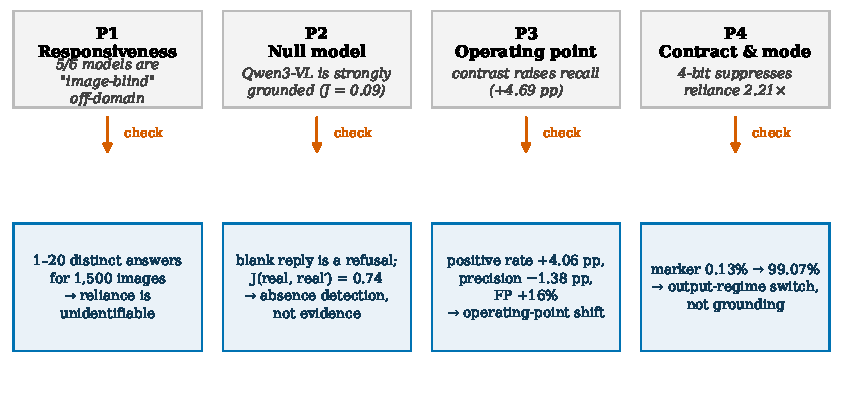
\includegraphics[width=\textwidth]{figures/fig01_four_reversals.pdf}
\caption{The four preconditions and the four reversals they prevent. Each top box is the conclusion a reader would draw from the reported statistic alone; each bottom box is the conclusion after the check.}
\label{fig:reversals}
\end{figure}
